The diverse information provided by \cockpit can help users and researchers in
many ways, some of which, just like for a traditional debugger, only become
apparent in practical use. In this section, we present a few motivating
examples, selecting specific instruments and scenarios in which they are
practically useful. Specifically, we show that \cockpit can help the user
discern between, and thus fix, common training bugs
(\Cref{cockpit::sec:misscaled_data_exp,cockpit::sec:vanishing_gradient_exp}) that are otherwise
hard to distinguish as they lead to the same failure: bad training. We
demonstrate that \cockpit can guide practitioners to choose efficient
hyperparameters \emph{within a single training run}
(\Cref{cockpit::sec:vanishing_gradient_exp,cockpit::sec:alpha_exp}). Finally, we highlight that
\cockpit's instruments can provide research insights about the optimization
process (\Cref{cockpit::sec:alpha_exp}). Our empirical findings are demonstrated on
problems from the \deepobs \citep{schneider2019deepobs} benchmark collection.

\subsection{Incorrectly Scaled Data}\label{cockpit::sec:misscaled_data_exp}
One prominent source of bugs is the data pipeline. To pick a relatively simple
example: for standard optimizers to work at their usual learning rates, network
inputs must be standardized (\ie~between zero and one, or have zero mean and
unit variance \citep[\eg][]{bengio2012neural}). If the user forgets to do this,
optimizer performance is likely to degrade. It can be difficult to identify the
source of this problem as it does not cause obvious failures, \texttt{NaN} or
\texttt{Inf} gradients, \etc. We now construct a semi-realistic example, to show
how using \cockpit can help diagnose this problem upon observing slow training
performance.

By default\sidenote{See the documentation, available at
  \href{https://www.cs.toronto.edu/~kriz/cifar.html}{\texttt{cs.toronto.edu/\textasciitilde
      kriz/cifar.html}}}, the popular image datasets \cifartenhun
\citep{krizhevsky2009learning} are provided as \numpy \citep{harris2020array}
arrays that consist of integers in the interval $[0,255]$. This \emph{raw} data,
instead of the widely used version with floats in $[0,1]$, changes the data
scale and thus the gradients by a factor of $255$. Therefore, the optimizer's
optimal learning rate is scaled as well. In other words, the default parameters
of popular optimization methods may not work well anymore, or good
hyperparameters may take extreme values. Even if the user directly inspects the
training images, this may not be apparent
(\Cref{cockpit::fig:data-pre-processing}). But the gradient histogram instrument
of \cockpit, which has a deliberate default plotting range around $[-1,1]$ to
highlight such problems, immediately and prominently shows that there is an
issue.

\begin{figure}
%	 pgfplots style "prerocessingexperimentdefault"
		\pgfkeys{/pgfplots/preprocessingexperimentdefault/.style={
				width=\linewidth,
				height=1.4\linewidth,
				every axis plot/.append style={line width = 1.2pt},
				tick pos = left,
				xmajorticks = true,
				ymajorticks = true,
				ylabel near ticks,
				xlabel near ticks,
				xtick align = inside,
				ytick align = inside,
				legend cell align = left,
				legend columns = 1,
				legend pos = south east,
				legend style = {
					fill opacity = 0.9,
					text opacity = 1,
					font = \small,
				},
				xticklabel style = {font = \small, inner xsep = -5ex},
				xlabel style = {font = \small},
				axis line style = {black},
				yticklabel style = {font = \small, inner ysep = -4ex},
				ylabel style = {font = \small},
				title style = {font = \small, inner ysep = -3ex},
				grid = major,
				grid style = {dashed}
			}
		}
	
	\centering
	\begin{subfigure}[t]{0.46\textwidth}
		\begin{minipage}{.49\textwidth}
			\Cshadowbox{
\includegraphics[width = .35\textwidth]{fig/06_preprocessing/fig_samples/cifar10raw_3c3d_sample_00.png}}
			\Cshadowbox{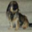
\includegraphics[width = .35\textwidth]{fig/06_preprocessing/fig_samples/cifar10raw_3c3d_sample_01.png}}
	
			\Cshadowbox{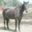
\includegraphics[width = .35\textwidth]{fig/06_preprocessing/fig_samples/cifar10raw_3c3d_sample_02.png}}
			\Cshadowbox{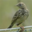
\includegraphics[width = .35\textwidth]{fig/06_preprocessing/fig_samples/cifar10raw_3c3d_sample_03.png}}
		\end{minipage}
		\begin{minipage}{.49\textwidth}
			\centering
			%			 customize "zmystyle" as you wish
			\pgfkeys{/pgfplots/zmystyle/.style={preprocessingexperimentdefault,
					ylabel={Gradient Element}
			}}
			\vspace{1.4\baselineskip}
			% This file was created by tikzplotlib v0.9.8.
\begin{tikzpicture}

\definecolor{color0}{rgb}{0.12156862745098,0.466666666666667,0.705882352941177}

\begin{axis}[
axis line style={white},
log basis x={10},
tick align=outside,
xmajorticks=false,
xmin=0.9, xmax=239494401.773689,
xmode=log,
xtick style={color=white!15!black},
ymajorticks=false,
ymin=-1.5, ymax=1.5,
zmystyle
]
\draw[draw=white,fill=color0,line width=0.04pt] (axis cs:0.9,-1.5) rectangle (axis cs:0.9,-1.42499995231628);
\draw[draw=white,fill=color0,line width=0.04pt] (axis cs:0.9,-1.42500007152557) rectangle (axis cs:0.9,-1.35000002384186);
\draw[draw=white,fill=color0,line width=0.04pt] (axis cs:0.9,-1.35000002384186) rectangle (axis cs:0.9,-1.27499997615814);
\draw[draw=white,fill=color0,line width=0.04pt] (axis cs:0.9,-1.27499997615814) rectangle (axis cs:0.9,-1.19999992847443);
\draw[draw=white,fill=color0,line width=0.04pt] (axis cs:0.9,-1.20000004768372) rectangle (axis cs:0.9,-1.125);
\draw[draw=white,fill=color0,line width=0.04pt] (axis cs:0.9,-1.125) rectangle (axis cs:0.9,-1.04999995231628);
\draw[draw=white,fill=color0,line width=0.04pt] (axis cs:0.9,-1.04999995231628) rectangle (axis cs:0.9,-0.974999904632568);
\draw[draw=white,fill=color0,line width=0.04pt] (axis cs:0.9,-0.975000023841858) rectangle (axis cs:0.9,-0.899999976158142);
\draw[draw=white,fill=color0,line width=0.04pt] (axis cs:0.9,-0.899999976158142) rectangle (axis cs:0.9,-0.824999928474426);
\draw[draw=white,fill=color0,line width=0.04pt] (axis cs:0.9,-0.825000047683716) rectangle (axis cs:0.9,-0.75);
\draw[draw=white,fill=color0,line width=0.04pt] (axis cs:0.9,-0.75) rectangle (axis cs:0.9,-0.674999952316284);
\draw[draw=white,fill=color0,line width=0.04pt] (axis cs:0.9,-0.674999952316284) rectangle (axis cs:0.9,-0.599999904632568);
\draw[draw=white,fill=color0,line width=0.04pt] (axis cs:0.9,-0.600000023841858) rectangle (axis cs:0.9,-0.524999976158142);
\draw[draw=white,fill=color0,line width=0.04pt] (axis cs:0.9,-0.524999976158142) rectangle (axis cs:0.9,-0.449999928474426);
\draw[draw=white,fill=color0,line width=0.04pt] (axis cs:0.9,-0.449999988079071) rectangle (axis cs:0.9,-0.374999940395355);
\draw[draw=white,fill=color0,line width=0.04pt] (axis cs:0.9,-0.374999970197678) rectangle (axis cs:0.9,-0.299999922513962);
\draw[draw=white,fill=color0,line width=0.04pt] (axis cs:0.9,-0.299999982118607) rectangle (axis cs:15.9,-0.224999934434891);
\draw[draw=white,fill=color0,line width=0.04pt] (axis cs:0.9,-0.224999964237213) rectangle (axis cs:755.9,-0.149999916553497);
\draw[draw=white,fill=color0,line width=0.04pt] (axis cs:0.9,-0.149999968707561) rectangle (axis cs:12866.9,-0.0749999210238457);
\draw[draw=white,fill=color0,line width=0.04pt] (axis cs:0.9,-0.075000025331974) rectangle (axis cs:95082889.9,2.23517417907715e-08);
\draw[draw=white,fill=color0,line width=0.04pt] (axis cs:0.9,-8.19563865661621e-08) rectangle (axis cs:19475047.9,0.0749999657273293);
\draw[draw=white,fill=color0,line width=0.04pt] (axis cs:0.9,0.0749999210238457) rectangle (axis cs:14378.9,0.149999968707561);
\draw[draw=white,fill=color0,line width=0.04pt] (axis cs:0.9,0.149999916553497) rectangle (axis cs:794.9,0.224999964237213);
\draw[draw=white,fill=color0,line width=0.04pt] (axis cs:0.9,0.224999934434891) rectangle (axis cs:8.9,0.299999982118607);
\draw[draw=white,fill=color0,line width=0.04pt] (axis cs:0.9,0.299999922513962) rectangle (axis cs:0.9,0.374999970197678);
\draw[draw=white,fill=color0,line width=0.04pt] (axis cs:0.9,0.374999940395355) rectangle (axis cs:0.9,0.449999988079071);
\draw[draw=white,fill=color0,line width=0.04pt] (axis cs:0.9,0.449999928474426) rectangle (axis cs:0.9,0.524999976158142);
\draw[draw=white,fill=color0,line width=0.04pt] (axis cs:0.9,0.524999976158142) rectangle (axis cs:0.9,0.600000023841858);
\draw[draw=white,fill=color0,line width=0.04pt] (axis cs:0.9,0.599999904632568) rectangle (axis cs:0.9,0.674999952316284);
\draw[draw=white,fill=color0,line width=0.04pt] (axis cs:0.9,0.674999952316284) rectangle (axis cs:0.9,0.75);
\draw[draw=white,fill=color0,line width=0.04pt] (axis cs:0.9,0.75) rectangle (axis cs:0.9,0.825000047683716);
\draw[draw=white,fill=color0,line width=0.04pt] (axis cs:0.9,0.824999928474426) rectangle (axis cs:30.9,0.899999976158142);
\draw[draw=white,fill=color0,line width=0.04pt] (axis cs:0.9,0.899999976158142) rectangle (axis cs:98.9,0.975000023841858);
\draw[draw=white,fill=color0,line width=0.04pt] (axis cs:0.9,0.974999904632568) rectangle (axis cs:0.9,1.04999995231628);
\draw[draw=white,fill=color0,line width=0.04pt] (axis cs:0.9,1.04999995231628) rectangle (axis cs:0.9,1.125);
\draw[draw=white,fill=color0,line width=0.04pt] (axis cs:0.9,1.125) rectangle (axis cs:0.9,1.20000004768372);
\draw[draw=white,fill=color0,line width=0.04pt] (axis cs:0.9,1.19999992847443) rectangle (axis cs:0.9,1.27499997615814);
\draw[draw=white,fill=color0,line width=0.04pt] (axis cs:0.9,1.27499997615814) rectangle (axis cs:0.9,1.35000002384186);
\draw[draw=white,fill=color0,line width=0.04pt] (axis cs:0.9,1.35000002384186) rectangle (axis cs:0.9,1.42500007152557);
\draw[draw=white,fill=color0,line width=0.04pt] (axis cs:0.9,1.42499995231628) rectangle (axis cs:0.9,1.5);
\end{axis}

\end{tikzpicture}

		\end{minipage}
		\caption{Normalized Data}
		\label{fig:data-pre-processing_norm}
	\end{subfigure}
	\hfill
	\begin{subfigure}[t]{0.46\textwidth}
		\begin{minipage}{.49\textwidth}
			\Cshadowbox{
\includegraphics[width = .35\textwidth]{fig/06_preprocessing/fig_samples/cifar10scale255_3c3d_sample_00.png}}
			\Cshadowbox{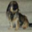
\includegraphics[width = .35\textwidth]{fig/06_preprocessing/fig_samples/cifar10scale255_3c3d_sample_01.png}}
			
			\Cshadowbox{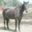
\includegraphics[width = .35\textwidth]{fig/06_preprocessing/fig_samples/cifar10scale255_3c3d_sample_02.png}}
			\Cshadowbox{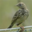
\includegraphics[width = .35\textwidth]{fig/06_preprocessing/fig_samples/cifar10scale255_3c3d_sample_03.png}}
		\end{minipage}
		\begin{minipage}{.49\textwidth}
			\centering
%			 customize "zmystyle" as you wish
			\pgfkeys{/pgfplots/zmystyle/.style={preprocessingexperimentdefault,
					ylabel={Gradient Element}
			}}
			\vspace{1.4\baselineskip}
			% This file was created by tikzplotlib v0.9.8.
\begin{tikzpicture}

\definecolor{color0}{rgb}{1,0.498039215686275,0.0549019607843137}

\begin{axis}[
axis line style={white},
log basis x={10},
tick align=outside,
xmajorticks=false,
xmin=0.9, xmax=199565229.367149,
xmode=log,
xtick style={color=white!15!black},
ymajorticks=false,
ymin=-1.5, ymax=1.5,
zmystyle
]
\draw[draw=white,fill=color0,line width=0.04pt] (axis cs:0.9,-1.5) rectangle (axis cs:6792656.9,-1.42499995231628);
\draw[draw=white,fill=color0,line width=0.04pt] (axis cs:0.9,-1.42500007152557) rectangle (axis cs:304537.9,-1.35000002384186);
\draw[draw=white,fill=color0,line width=0.04pt] (axis cs:0.9,-1.35000002384186) rectangle (axis cs:322920.9,-1.27499997615814);
\draw[draw=white,fill=color0,line width=0.04pt] (axis cs:0.9,-1.27499997615814) rectangle (axis cs:342177.9,-1.19999992847443);
\draw[draw=white,fill=color0,line width=0.04pt] (axis cs:0.9,-1.20000004768372) rectangle (axis cs:365697.9,-1.125);
\draw[draw=white,fill=color0,line width=0.04pt] (axis cs:0.9,-1.125) rectangle (axis cs:389812.9,-1.04999995231628);
\draw[draw=white,fill=color0,line width=0.04pt] (axis cs:0.9,-1.04999995231628) rectangle (axis cs:417003.9,-0.974999904632568);
\draw[draw=white,fill=color0,line width=0.04pt] (axis cs:0.9,-0.975000023841858) rectangle (axis cs:446173.9,-0.899999976158142);
\draw[draw=white,fill=color0,line width=0.04pt] (axis cs:0.9,-0.899999976158142) rectangle (axis cs:476860.9,-0.824999928474426);
\draw[draw=white,fill=color0,line width=0.04pt] (axis cs:0.9,-0.825000047683716) rectangle (axis cs:514596.9,-0.75);
\draw[draw=white,fill=color0,line width=0.04pt] (axis cs:0.9,-0.75) rectangle (axis cs:555044.9,-0.674999952316284);
\draw[draw=white,fill=color0,line width=0.04pt] (axis cs:0.9,-0.674999952316284) rectangle (axis cs:601849.9,-0.599999904632568);
\draw[draw=white,fill=color0,line width=0.04pt] (axis cs:0.9,-0.600000023841858) rectangle (axis cs:653348.9,-0.524999976158142);
\draw[draw=white,fill=color0,line width=0.04pt] (axis cs:0.9,-0.524999976158142) rectangle (axis cs:715926.9,-0.449999928474426);
\draw[draw=white,fill=color0,line width=0.04pt] (axis cs:0.9,-0.449999988079071) rectangle (axis cs:790634.9,-0.374999940395355);
\draw[draw=white,fill=color0,line width=0.04pt] (axis cs:0.9,-0.374999970197678) rectangle (axis cs:880821.9,-0.299999922513962);
\draw[draw=white,fill=color0,line width=0.04pt] (axis cs:0.9,-0.299999982118607) rectangle (axis cs:996047.9,-0.224999934434891);
\draw[draw=white,fill=color0,line width=0.04pt] (axis cs:0.9,-0.224999964237213) rectangle (axis cs:1158251.9,-0.149999916553497);
\draw[draw=white,fill=color0,line width=0.04pt] (axis cs:0.9,-0.149999968707561) rectangle (axis cs:1410941.9,-0.0749999210238457);
\draw[draw=white,fill=color0,line width=0.04pt] (axis cs:0.9,-0.075000025331974) rectangle (axis cs:79921533.9,2.23517417907715e-08);
\draw[draw=white,fill=color0,line width=0.04pt] (axis cs:0.9,-8.19563865661621e-08) rectangle (axis cs:1965478.9,0.0749999657273293);
\draw[draw=white,fill=color0,line width=0.04pt] (axis cs:0.9,0.0749999210238457) rectangle (axis cs:1289789.9,0.149999968707561);
\draw[draw=white,fill=color0,line width=0.04pt] (axis cs:0.9,0.149999916553497) rectangle (axis cs:1043170.9,0.224999964237213);
\draw[draw=white,fill=color0,line width=0.04pt] (axis cs:0.9,0.224999934434891) rectangle (axis cs:885990.9,0.299999982118607);
\draw[draw=white,fill=color0,line width=0.04pt] (axis cs:0.9,0.299999922513962) rectangle (axis cs:771669.9,0.374999970197678);
\draw[draw=white,fill=color0,line width=0.04pt] (axis cs:0.9,0.374999940395355) rectangle (axis cs:683281.9,0.449999988079071);
\draw[draw=white,fill=color0,line width=0.04pt] (axis cs:0.9,0.449999928474426) rectangle (axis cs:610831.9,0.524999976158142);
\draw[draw=white,fill=color0,line width=0.04pt] (axis cs:0.9,0.524999976158142) rectangle (axis cs:553292.9,0.600000023841858);
\draw[draw=white,fill=color0,line width=0.04pt] (axis cs:0.9,0.599999904632568) rectangle (axis cs:502804.9,0.674999952316284);
\draw[draw=white,fill=color0,line width=0.04pt] (axis cs:0.9,0.674999952316284) rectangle (axis cs:461496.9,0.75);
\draw[draw=white,fill=color0,line width=0.04pt] (axis cs:0.9,0.75) rectangle (axis cs:423747.9,0.825000047683716);
\draw[draw=white,fill=color0,line width=0.04pt] (axis cs:0.9,0.824999928474426) rectangle (axis cs:392145.9,0.899999976158142);
\draw[draw=white,fill=color0,line width=0.04pt] (axis cs:0.9,0.899999976158142) rectangle (axis cs:363396.9,0.975000023841858);
\draw[draw=white,fill=color0,line width=0.04pt] (axis cs:0.9,0.974999904632568) rectangle (axis cs:335621.9,1.04999995231628);
\draw[draw=white,fill=color0,line width=0.04pt] (axis cs:0.9,1.04999995231628) rectangle (axis cs:312992.9,1.125);
\draw[draw=white,fill=color0,line width=0.04pt] (axis cs:0.9,1.125) rectangle (axis cs:291497.9,1.20000004768372);
\draw[draw=white,fill=color0,line width=0.04pt] (axis cs:0.9,1.19999992847443) rectangle (axis cs:273292.9,1.27499997615814);
\draw[draw=white,fill=color0,line width=0.04pt] (axis cs:0.9,1.27499997615814) rectangle (axis cs:255338.9,1.35000002384186);
\draw[draw=white,fill=color0,line width=0.04pt] (axis cs:0.9,1.35000002384186) rectangle (axis cs:240647.9,1.42500007152557);
\draw[draw=white,fill=color0,line width=0.04pt] (axis cs:0.9,1.42499995231628) rectangle (axis cs:4873580.9,1.5);
\end{axis}

\end{tikzpicture}

		\end{minipage}
		\caption{Raw Data}
		\label{fig:data-pre-processing_raw}
	\end{subfigure}
	\caption{\textbf{Same inputs, different gradients; Catching data 
	    bugs with \cockpittitle.} (a) \emph{normalized} ($[0, 1]$) and (b)
    	\emph{raw} $([0, 255])$ images look identical in auto-scaled
	    front-ends like \matplotlib's \texttt{imshow}. The gradient distribution on
	    the \threecthreed model, however, is crucially affected by this
	    scaling.}
	\label{fig:data-pre-processing}
\end{figure}

%%% Local Variables:
%%% mode: latex
%%% TeX-master: "../cockpit_paper"
%%% End:


Of course, this particular data is only a placeholder for real practical data
sets. While this problem may not frequently arise in the highly pre-processed,
packaged \cifarten, it is not a rare problem for practitioners who work with
their personal datasets. This is particularly likely in domains outside
standard computer vision, \eg when working with mixed-type data without obvious
natural scales.

\subsection{Vanishing Gradients}\label{cockpit::sec:vanishing_gradient_exp}

The model itself can be a source of training bugs. As before, such problems
mostly arise with novel datasets, where well-working architectures are unknown.
The following example shows how even small (in terms of code) model
modifications may severely harm the training.

\Cref{cockpit::fig:layerwise-experiment_net} shows the distribution of gradient values of
two different network architectures in blue and orange. Although the blue model
trains considerably better than the orange one, their gradient distributions
look quite similar. The difference becomes evident when inspecting the histogram
\emph{layer-wise}. We can see that multiple layers have a degenerated gradient
distribution with many elements being practically zero (see
\Cref{cockpit::fig:layerwise-experiment_layers}, bottom row). Since the fully connected
layers close to the output have far more parameters (a typical pattern of
convolutional networks), they dominate the network-wide histogram. This obscures
that a major part of the model is effectively unable to train.

\begin{figure}
%	 pgfplots style "layerwiseexperimentdefault"
	  \pgfkeys{/pgfplots/layerwiseexperimentdefault/.style={
	      width=\linewidth,
	      height=0.13\textheight,
	      every axis plot/.append style={line width = 1.2pt},
	      tick pos = left,
	      xmajorticks = true,
	      ymajorticks = true,
	      ylabel near ticks,
	      xlabel near ticks,
	      xtick align = inside,
	      ytick align = inside,
	      ytick={-1,0,1},
	      legend cell align = left,
	      legend columns = 1,
	      legend pos = south east,
	      legend style = {
	        fill opacity = 0.9,
	        text opacity = 1,
	        font = \small,
	      },
	      xticklabel style = {font = \small, inner xsep = -5ex},
	      xlabel style = {font = \small},
	      axis line style = {black},
	      yticklabel style = {font = \small, inner ysep = -4ex},
	      ylabel style = {font = \small},
	      title style = {font = \small, inner ysep = -3ex},
	      grid = major,
	      grid style = {dashed}
	    }
	  }
	
	\centering
	\begin{subfigure}[t]{0.4\textwidth}
%		 customize "zmystyle" as you wish
		\pgfkeys{/pgfplots/zmystyle/.style={layerwiseexperimentdefault,
		   title = {Network}, ylabel=Gradient\\Element, ylabel style={align=left}, xticklabels = {}
		 }}
		% This file was created by tikzplotlib v0.9.8.
\begin{tikzpicture}

\definecolor{color0}{rgb}{0.12156862745098,0.466666666666667,0.705882352941177}

\begin{axis}[
axis line style={white},
log basis x={10},
tick align=outside,
xmajorticks=false,
xmin=0.9, xmax=233063278.37446,
xmode=log,
xtick style={color=white!15!black},
ymajorticks=false,
ymin=-1.1000000834465, ymax=1.1000000834465,
zmystyle
]
\draw[draw=white,fill=color0,line width=0.02pt] (axis cs:0.9,-1.1000000834465) rectangle (axis cs:0.9,-0.990000069141388);
\draw[draw=white,fill=color0,line width=0.02pt] (axis cs:0.9,-0.990000009536743) rectangle (axis cs:0.9,-0.879999995231628);
\draw[draw=white,fill=color0,line width=0.02pt] (axis cs:0.9,-0.880000054836273) rectangle (axis cs:0.9,-0.770000040531158);
\draw[draw=white,fill=color0,line width=0.02pt] (axis cs:0.9,-0.770000040531158) rectangle (axis cs:0.9,-0.660000026226044);
\draw[draw=white,fill=color0,line width=0.02pt] (axis cs:0.9,-0.660000026226044) rectangle (axis cs:0.9,-0.550000011920929);
\draw[draw=white,fill=color0,line width=0.02pt] (axis cs:0.9,-0.550000011920929) rectangle (axis cs:0.9,-0.439999997615814);
\draw[draw=white,fill=color0,line width=0.02pt] (axis cs:0.9,-0.440000057220459) rectangle (axis cs:23.9,-0.330000042915344);
\draw[draw=white,fill=color0,line width=0.02pt] (axis cs:0.9,-0.330000042915344) rectangle (axis cs:868.9,-0.220000028610229);
\draw[draw=white,fill=color0,line width=0.02pt] (axis cs:0.9,-0.220000028610229) rectangle (axis cs:38909.9,-0.110000014305115);
\draw[draw=white,fill=color0,line width=0.02pt] (axis cs:0.9,-0.110000006854534) rectangle (axis cs:92649650.9,7.45058059692383e-09);
\draw[draw=white,fill=color0,line width=0.02pt] (axis cs:0.9,2.23517417907715e-08) rectangle (axis cs:21858861.9,0.110000036656857);
\draw[draw=white,fill=color0,line width=0.02pt] (axis cs:0.9,0.110000014305115) rectangle (axis cs:35123.9,0.220000028610229);
\draw[draw=white,fill=color0,line width=0.02pt] (axis cs:0.9,0.220000028610229) rectangle (axis cs:2220.9,0.330000042915344);
\draw[draw=white,fill=color0,line width=0.02pt] (axis cs:0.9,0.330000042915344) rectangle (axis cs:686.9,0.440000057220459);
\draw[draw=white,fill=color0,line width=0.02pt] (axis cs:0.9,0.439999997615814) rectangle (axis cs:276.9,0.550000011920929);
\draw[draw=white,fill=color0,line width=0.02pt] (axis cs:0.9,0.550000011920929) rectangle (axis cs:95.9,0.660000026226044);
\draw[draw=white,fill=color0,line width=0.02pt] (axis cs:0.9,0.660000026226044) rectangle (axis cs:27.9,0.770000040531158);
\draw[draw=white,fill=color0,line width=0.02pt] (axis cs:0.9,0.770000040531158) rectangle (axis cs:25.9,0.880000054836273);
\draw[draw=white,fill=color0,line width=0.02pt] (axis cs:0.9,0.879999995231628) rectangle (axis cs:117.9,0.990000009536743);
\draw[draw=white,fill=color0,line width=0.02pt] (axis cs:0.9,0.990000069141388) rectangle (axis cs:0.9,1.1000000834465);
\end{axis}

\end{tikzpicture}

		
		\vspace{-0.1cm}
%		customize "zmystyle" as you wish
		\pgfkeys{/pgfplots/zmystyle/.style={layerwiseexperimentdefault,
		   ylabel=Gradient\\Element, ylabel style={align=left}
		 }}
		% This file was created by tikzplotlib v0.9.8.
\begin{tikzpicture}

\definecolor{color0}{rgb}{1,0.498039215686275,0.0549019607843137}

\begin{axis}[
axis line style={white},
log basis x={10},
tick align=outside,
xmajorticks=false,
xmin=0.9, xmax=141796339.435146,
xmode=log,
xtick style={color=white!15!black},
ymajorticks=false,
ymin=-1.1000000834465, ymax=1.1000000834465,
zmystyle
]
\draw[draw=white,fill=color0,line width=0.02pt] (axis cs:0.9,-1.1000000834465) rectangle (axis cs:0.9,-0.990000069141388);
\draw[draw=white,fill=color0,line width=0.02pt] (axis cs:0.9,-0.990000009536743) rectangle (axis cs:0.9,-0.879999995231628);
\draw[draw=white,fill=color0,line width=0.02pt] (axis cs:0.9,-0.880000054836273) rectangle (axis cs:0.9,-0.770000040531158);
\draw[draw=white,fill=color0,line width=0.02pt] (axis cs:0.9,-0.770000040531158) rectangle (axis cs:0.9,-0.660000026226044);
\draw[draw=white,fill=color0,line width=0.02pt] (axis cs:0.9,-0.660000026226044) rectangle (axis cs:0.9,-0.550000011920929);
\draw[draw=white,fill=color0,line width=0.02pt] (axis cs:0.9,-0.550000011920929) rectangle (axis cs:0.9,-0.439999997615814);
\draw[draw=white,fill=color0,line width=0.02pt] (axis cs:0.9,-0.440000057220459) rectangle (axis cs:116.9,-0.330000042915344);
\draw[draw=white,fill=color0,line width=0.02pt] (axis cs:0.9,-0.330000042915344) rectangle (axis cs:7658.9,-0.220000028610229);
\draw[draw=white,fill=color0,line width=0.02pt] (axis cs:0.9,-0.220000028610229) rectangle (axis cs:41443.9,-0.110000014305115);
\draw[draw=white,fill=color0,line width=0.02pt] (axis cs:0.9,-0.110000006854534) rectangle (axis cs:57718038.9,7.45058059692383e-09);
\draw[draw=white,fill=color0,line width=0.02pt] (axis cs:0.9,2.23517417907715e-08) rectangle (axis cs:56786753.9,0.110000036656857);
\draw[draw=white,fill=color0,line width=0.02pt] (axis cs:0.9,0.110000014305115) rectangle (axis cs:1065.9,0.220000028610229);
\draw[draw=white,fill=color0,line width=0.02pt] (axis cs:0.9,0.220000028610229) rectangle (axis cs:5071.9,0.330000042915344);
\draw[draw=white,fill=color0,line width=0.02pt] (axis cs:0.9,0.330000042915344) rectangle (axis cs:8560.9,0.440000057220459);
\draw[draw=white,fill=color0,line width=0.02pt] (axis cs:0.9,0.439999997615814) rectangle (axis cs:10133.9,0.550000011920929);
\draw[draw=white,fill=color0,line width=0.02pt] (axis cs:0.9,0.550000011920929) rectangle (axis cs:5885.9,0.660000026226044);
\draw[draw=white,fill=color0,line width=0.02pt] (axis cs:0.9,0.660000026226044) rectangle (axis cs:1847.9,0.770000040531158);
\draw[draw=white,fill=color0,line width=0.02pt] (axis cs:0.9,0.770000040531158) rectangle (axis cs:203.9,0.880000054836273);
\draw[draw=white,fill=color0,line width=0.02pt] (axis cs:0.9,0.879999995231628) rectangle (axis cs:108.9,0.990000009536743);
\draw[draw=white,fill=color0,line width=0.02pt] (axis cs:0.9,0.990000069141388) rectangle (axis cs:0.9,1.1000000834465);
\end{axis}

\end{tikzpicture}

		\caption{Network Histogram}
		\label{fig:layerwise-experiment_net}
	\end{subfigure}
	\hfill
	\begin{subfigure}[t]{0.57\textwidth}
		    \pgfkeys{/pgfplots/layerwiseexperimentdefaultparameters/.style={
		        layerwiseexperimentdefault,
		        ylabel={},
		        ylabel style = {inner ysep = -4ex},
		        yticklabels={},
		        width=0.45\textwidth,
		      }
		    }
		    \hfill%
		    \pgfkeys{/pgfplots/zmystyle/.style={layerwiseexperimentdefaultparameters,
		        title={Parameter 0}, xticklabels = {},}}%
		    % This file was created by tikzplotlib v0.9.8.
\begin{tikzpicture}

\definecolor{color0}{rgb}{0.12156862745098,0.466666666666667,0.705882352941177}

\begin{axis}[
axis line style={white},
log basis x={10},
tick align=outside,
xmajorticks=false,
xmin=0.9, xmax=570529.892272652,
xmode=log,
xtick style={color=white!15!black},
ymajorticks=false,
ymin=-1.1000000834465, ymax=1.1000000834465,
zmystyle
]
\draw[draw=white,fill=color0,line width=0.02pt] (axis cs:0.9,-1.1000000834465) rectangle (axis cs:0.9,-0.990000069141388);
\draw[draw=white,fill=color0,line width=0.02pt] (axis cs:0.9,-0.990000009536743) rectangle (axis cs:0.9,-0.879999995231628);
\draw[draw=white,fill=color0,line width=0.02pt] (axis cs:0.9,-0.880000054836273) rectangle (axis cs:0.9,-0.770000040531158);
\draw[draw=white,fill=color0,line width=0.02pt] (axis cs:0.9,-0.770000040531158) rectangle (axis cs:0.9,-0.660000026226044);
\draw[draw=white,fill=color0,line width=0.02pt] (axis cs:0.9,-0.660000026226044) rectangle (axis cs:0.9,-0.550000011920929);
\draw[draw=white,fill=color0,line width=0.02pt] (axis cs:0.9,-0.550000011920929) rectangle (axis cs:0.9,-0.439999997615814);
\draw[draw=white,fill=color0,line width=0.02pt] (axis cs:0.9,-0.440000057220459) rectangle (axis cs:23.9,-0.330000042915344);
\draw[draw=white,fill=color0,line width=0.02pt] (axis cs:0.9,-0.330000042915344) rectangle (axis cs:528.9,-0.220000028610229);
\draw[draw=white,fill=color0,line width=0.02pt] (axis cs:0.9,-0.220000028610229) rectangle (axis cs:11638.9,-0.110000014305115);
\draw[draw=white,fill=color0,line width=0.02pt] (axis cs:0.9,-0.110000006854534) rectangle (axis cs:301988.9,7.45058059692383e-09);
\draw[draw=white,fill=color0,line width=0.02pt] (axis cs:0.9,2.23517417907715e-08) rectangle (axis cs:288675.9,0.110000036656857);
\draw[draw=white,fill=color0,line width=0.02pt] (axis cs:0.9,0.110000014305115) rectangle (axis cs:11178.9,0.220000028610229);
\draw[draw=white,fill=color0,line width=0.02pt] (axis cs:0.9,0.220000028610229) rectangle (axis cs:370.9,0.330000042915344);
\draw[draw=white,fill=color0,line width=0.02pt] (axis cs:0.9,0.330000042915344) rectangle (axis cs:0.9,0.440000057220459);
\draw[draw=white,fill=color0,line width=0.02pt] (axis cs:0.9,0.439999997615814) rectangle (axis cs:0.9,0.550000011920929);
\draw[draw=white,fill=color0,line width=0.02pt] (axis cs:0.9,0.550000011920929) rectangle (axis cs:0.9,0.660000026226044);
\draw[draw=white,fill=color0,line width=0.02pt] (axis cs:0.9,0.660000026226044) rectangle (axis cs:0.9,0.770000040531158);
\draw[draw=white,fill=color0,line width=0.02pt] (axis cs:0.9,0.770000040531158) rectangle (axis cs:0.9,0.880000054836273);
\draw[draw=white,fill=color0,line width=0.02pt] (axis cs:0.9,0.879999995231628) rectangle (axis cs:0.9,0.990000009536743);
\draw[draw=white,fill=color0,line width=0.02pt] (axis cs:0.9,0.990000069141388) rectangle (axis cs:0.9,1.1000000834465);
\end{axis}

\end{tikzpicture}

		    \hfill
		    \pgfkeys{/pgfplots/zmystyle/.style={layerwiseexperimentdefaultparameters,
		        title={Parameter 4}, xticklabels = {},}}%
		    % This file was created by tikzplotlib v0.9.8.
\begin{tikzpicture}

\definecolor{color0}{rgb}{0.12156862745098,0.466666666666667,0.705882352941177}

\begin{axis}[
axis line style={white},
log basis x={10},
tick align=outside,
xmajorticks=false,
xmin=0.9, xmax=21044199.0041348,
xmode=log,
xtick style={color=white!15!black},
ymajorticks=false,
ymin=-1.1000000834465, ymax=1.1000000834465,
zmystyle
]
\draw[draw=white,fill=color0,line width=0.02pt] (axis cs:0.9,-1.1000000834465) rectangle (axis cs:0.9,-0.990000069141388);
\draw[draw=white,fill=color0,line width=0.02pt] (axis cs:0.9,-0.990000009536743) rectangle (axis cs:0.9,-0.879999995231628);
\draw[draw=white,fill=color0,line width=0.02pt] (axis cs:0.9,-0.880000054836273) rectangle (axis cs:0.9,-0.770000040531158);
\draw[draw=white,fill=color0,line width=0.02pt] (axis cs:0.9,-0.770000040531158) rectangle (axis cs:0.9,-0.660000026226044);
\draw[draw=white,fill=color0,line width=0.02pt] (axis cs:0.9,-0.660000026226044) rectangle (axis cs:0.9,-0.550000011920929);
\draw[draw=white,fill=color0,line width=0.02pt] (axis cs:0.9,-0.550000011920929) rectangle (axis cs:0.9,-0.439999997615814);
\draw[draw=white,fill=color0,line width=0.02pt] (axis cs:0.9,-0.440000057220459) rectangle (axis cs:0.9,-0.330000042915344);
\draw[draw=white,fill=color0,line width=0.02pt] (axis cs:0.9,-0.330000042915344) rectangle (axis cs:242.9,-0.220000028610229);
\draw[draw=white,fill=color0,line width=0.02pt] (axis cs:0.9,-0.220000028610229) rectangle (axis cs:12057.9,-0.110000014305115);
\draw[draw=white,fill=color0,line width=0.02pt] (axis cs:0.9,-0.110000006854534) rectangle (axis cs:9380648.9,7.45058059692383e-09);
\draw[draw=white,fill=color0,line width=0.02pt] (axis cs:0.9,2.23517417907715e-08) rectangle (axis cs:4752253.9,0.110000036656857);
\draw[draw=white,fill=color0,line width=0.02pt] (axis cs:0.9,0.110000014305115) rectangle (axis cs:10313.9,0.220000028610229);
\draw[draw=white,fill=color0,line width=0.02pt] (axis cs:0.9,0.220000028610229) rectangle (axis cs:256.9,0.330000042915344);
\draw[draw=white,fill=color0,line width=0.02pt] (axis cs:0.9,0.330000042915344) rectangle (axis cs:7.9,0.440000057220459);
\draw[draw=white,fill=color0,line width=0.02pt] (axis cs:0.9,0.439999997615814) rectangle (axis cs:0.9,0.550000011920929);
\draw[draw=white,fill=color0,line width=0.02pt] (axis cs:0.9,0.550000011920929) rectangle (axis cs:0.9,0.660000026226044);
\draw[draw=white,fill=color0,line width=0.02pt] (axis cs:0.9,0.660000026226044) rectangle (axis cs:0.9,0.770000040531158);
\draw[draw=white,fill=color0,line width=0.02pt] (axis cs:0.9,0.770000040531158) rectangle (axis cs:0.9,0.880000054836273);
\draw[draw=white,fill=color0,line width=0.02pt] (axis cs:0.9,0.879999995231628) rectangle (axis cs:0.9,0.990000009536743);
\draw[draw=white,fill=color0,line width=0.02pt] (axis cs:0.9,0.990000069141388) rectangle (axis cs:0.9,1.1000000834465);
\end{axis}

\end{tikzpicture}

		    \pgfkeys{/pgfplots/zmystyle/.style={layerwiseexperimentdefaultparameters,
		        title={Parameter 10}, xticklabels = {},}}%
		    \hfill
		    % This file was created by tikzplotlib v0.9.8.
\begin{tikzpicture}

\definecolor{color0}{rgb}{0.12156862745098,0.466666666666667,0.705882352941177}

\begin{axis}[
axis line style={white},
log basis x={10},
tick align=outside,
xmajorticks=false,
xmin=0.9, xmax=590238.132533874,
xmode=log,
xtick style={color=white!15!black},
ymajorticks=false,
ymin=-1.1000000834465, ymax=1.1000000834465,
zmystyle
]
\draw[draw=white,fill=color0,line width=0.02pt] (axis cs:0.9,-1.1000000834465) rectangle (axis cs:0.9,-0.990000069141388);
\draw[draw=white,fill=color0,line width=0.02pt] (axis cs:0.9,-0.990000009536743) rectangle (axis cs:0.9,-0.879999995231628);
\draw[draw=white,fill=color0,line width=0.02pt] (axis cs:0.9,-0.880000054836273) rectangle (axis cs:0.9,-0.770000040531158);
\draw[draw=white,fill=color0,line width=0.02pt] (axis cs:0.9,-0.770000040531158) rectangle (axis cs:0.9,-0.660000026226044);
\draw[draw=white,fill=color0,line width=0.02pt] (axis cs:0.9,-0.660000026226044) rectangle (axis cs:0.9,-0.550000011920929);
\draw[draw=white,fill=color0,line width=0.02pt] (axis cs:0.9,-0.550000011920929) rectangle (axis cs:0.9,-0.439999997615814);
\draw[draw=white,fill=color0,line width=0.02pt] (axis cs:0.9,-0.440000057220459) rectangle (axis cs:0.9,-0.330000042915344);
\draw[draw=white,fill=color0,line width=0.02pt] (axis cs:0.9,-0.330000042915344) rectangle (axis cs:2.9,-0.220000028610229);
\draw[draw=white,fill=color0,line width=0.02pt] (axis cs:0.9,-0.220000028610229) rectangle (axis cs:251.9,-0.110000014305115);
\draw[draw=white,fill=color0,line width=0.02pt] (axis cs:0.9,-0.110000006854534) rectangle (axis cs:311915.9,7.45058059692383e-09);
\draw[draw=white,fill=color0,line width=0.02pt] (axis cs:0.9,2.23517417907715e-08) rectangle (axis cs:9028.9,0.110000036656857);
\draw[draw=white,fill=color0,line width=0.02pt] (axis cs:0.9,0.110000014305115) rectangle (axis cs:3828.9,0.220000028610229);
\draw[draw=white,fill=color0,line width=0.02pt] (axis cs:0.9,0.220000028610229) rectangle (axis cs:1565.9,0.330000042915344);
\draw[draw=white,fill=color0,line width=0.02pt] (axis cs:0.9,0.330000042915344) rectangle (axis cs:679.9,0.440000057220459);
\draw[draw=white,fill=color0,line width=0.02pt] (axis cs:0.9,0.439999997615814) rectangle (axis cs:276.9,0.550000011920929);
\draw[draw=white,fill=color0,line width=0.02pt] (axis cs:0.9,0.550000011920929) rectangle (axis cs:95.9,0.660000026226044);
\draw[draw=white,fill=color0,line width=0.02pt] (axis cs:0.9,0.660000026226044) rectangle (axis cs:27.9,0.770000040531158);
\draw[draw=white,fill=color0,line width=0.02pt] (axis cs:0.9,0.770000040531158) rectangle (axis cs:13.9,0.880000054836273);
\draw[draw=white,fill=color0,line width=0.02pt] (axis cs:0.9,0.879999995231628) rectangle (axis cs:1.9,0.990000009536743);
\draw[draw=white,fill=color0,line width=0.02pt] (axis cs:0.9,0.990000069141388) rectangle (axis cs:0.9,1.1000000834465);
\end{axis}

\end{tikzpicture}

		    \hfill
		
		    \vspace{-0.1cm}\hspace{-0.25\baselineskip}\hfill
		    \pgfkeys{/pgfplots/zmystyle/.style={layerwiseexperimentdefaultparameters}}
		    % This file was created by tikzplotlib v0.9.8.
\begin{tikzpicture}

\definecolor{color0}{rgb}{1,0.498039215686275,0.0549019607843137}

\begin{axis}[
axis line style={white},
log basis x={10},
tick align=outside,
xmajorticks=false,
xmin=0.9, xmax=583677.09915469,
xmode=log,
xtick style={color=white!15!black},
ymajorticks=false,
ymin=-1.1000000834465, ymax=1.1000000834465,
zmystyle
]
\draw[draw=white,fill=color0,line width=0.02pt] (axis cs:0.9,-1.1000000834465) rectangle (axis cs:0.9,-0.990000069141388);
\draw[draw=white,fill=color0,line width=0.02pt] (axis cs:0.9,-0.990000009536743) rectangle (axis cs:0.9,-0.879999995231628);
\draw[draw=white,fill=color0,line width=0.02pt] (axis cs:0.9,-0.880000054836273) rectangle (axis cs:0.9,-0.770000040531158);
\draw[draw=white,fill=color0,line width=0.02pt] (axis cs:0.9,-0.770000040531158) rectangle (axis cs:0.9,-0.660000026226044);
\draw[draw=white,fill=color0,line width=0.02pt] (axis cs:0.9,-0.660000026226044) rectangle (axis cs:0.9,-0.550000011920929);
\draw[draw=white,fill=color0,line width=0.02pt] (axis cs:0.9,-0.550000011920929) rectangle (axis cs:0.9,-0.439999997615814);
\draw[draw=white,fill=color0,line width=0.02pt] (axis cs:0.9,-0.440000057220459) rectangle (axis cs:0.9,-0.330000042915344);
\draw[draw=white,fill=color0,line width=0.02pt] (axis cs:0.9,-0.330000042915344) rectangle (axis cs:0.9,-0.220000028610229);
\draw[draw=white,fill=color0,line width=0.02pt] (axis cs:0.9,-0.220000028610229) rectangle (axis cs:0.9,-0.110000014305115);
\draw[draw=white,fill=color0,line width=0.02pt] (axis cs:0.9,-0.110000006854534) rectangle (axis cs:305788.9,7.45058059692383e-09);
\draw[draw=white,fill=color0,line width=0.02pt] (axis cs:0.9,2.23517417907715e-08) rectangle (axis cs:308612.9,0.110000036656857);
\draw[draw=white,fill=color0,line width=0.02pt] (axis cs:0.9,0.110000014305115) rectangle (axis cs:0.9,0.220000028610229);
\draw[draw=white,fill=color0,line width=0.02pt] (axis cs:0.9,0.220000028610229) rectangle (axis cs:0.9,0.330000042915344);
\draw[draw=white,fill=color0,line width=0.02pt] (axis cs:0.9,0.330000042915344) rectangle (axis cs:0.9,0.440000057220459);
\draw[draw=white,fill=color0,line width=0.02pt] (axis cs:0.9,0.439999997615814) rectangle (axis cs:0.9,0.550000011920929);
\draw[draw=white,fill=color0,line width=0.02pt] (axis cs:0.9,0.550000011920929) rectangle (axis cs:0.9,0.660000026226044);
\draw[draw=white,fill=color0,line width=0.02pt] (axis cs:0.9,0.660000026226044) rectangle (axis cs:0.9,0.770000040531158);
\draw[draw=white,fill=color0,line width=0.02pt] (axis cs:0.9,0.770000040531158) rectangle (axis cs:0.9,0.880000054836273);
\draw[draw=white,fill=color0,line width=0.02pt] (axis cs:0.9,0.879999995231628) rectangle (axis cs:0.9,0.990000009536743);
\draw[draw=white,fill=color0,line width=0.02pt] (axis cs:0.9,0.990000069141388) rectangle (axis cs:0.9,1.1000000834465);
\end{axis}

\end{tikzpicture}

		    \hfill
		    % This file was created by tikzplotlib v0.9.8.
\begin{tikzpicture}

\definecolor{color0}{rgb}{1,0.498039215686275,0.0549019607843137}

\begin{axis}[
axis line style={white},
log basis x={10},
tick align=outside,
xmajorticks=false,
xmin=0.9, xmax=15871692.4114091,
xmode=log,
xtick style={color=white!15!black},
ymajorticks=false,
ymin=-1.1000000834465, ymax=1.1000000834465,
zmystyle
]
\draw[draw=white,fill=color0,line width=0.02pt] (axis cs:0.9,-1.1000000834465) rectangle (axis cs:0.9,-0.990000069141388);
\draw[draw=white,fill=color0,line width=0.02pt] (axis cs:0.9,-0.990000009536743) rectangle (axis cs:0.9,-0.879999995231628);
\draw[draw=white,fill=color0,line width=0.02pt] (axis cs:0.9,-0.880000054836273) rectangle (axis cs:0.9,-0.770000040531158);
\draw[draw=white,fill=color0,line width=0.02pt] (axis cs:0.9,-0.770000040531158) rectangle (axis cs:0.9,-0.660000026226044);
\draw[draw=white,fill=color0,line width=0.02pt] (axis cs:0.9,-0.660000026226044) rectangle (axis cs:0.9,-0.550000011920929);
\draw[draw=white,fill=color0,line width=0.02pt] (axis cs:0.9,-0.550000011920929) rectangle (axis cs:0.9,-0.439999997615814);
\draw[draw=white,fill=color0,line width=0.02pt] (axis cs:0.9,-0.440000057220459) rectangle (axis cs:0.9,-0.330000042915344);
\draw[draw=white,fill=color0,line width=0.02pt] (axis cs:0.9,-0.330000042915344) rectangle (axis cs:0.9,-0.220000028610229);
\draw[draw=white,fill=color0,line width=0.02pt] (axis cs:0.9,-0.220000028610229) rectangle (axis cs:0.9,-0.110000014305115);
\draw[draw=white,fill=color0,line width=0.02pt] (axis cs:0.9,-0.110000006854534) rectangle (axis cs:7170632.9,7.45058059692383e-09);
\draw[draw=white,fill=color0,line width=0.02pt] (axis cs:0.9,2.23517417907715e-08) rectangle (axis cs:6985144.9,0.110000036656857);
\draw[draw=white,fill=color0,line width=0.02pt] (axis cs:0.9,0.110000014305115) rectangle (axis cs:0.9,0.220000028610229);
\draw[draw=white,fill=color0,line width=0.02pt] (axis cs:0.9,0.220000028610229) rectangle (axis cs:0.9,0.330000042915344);
\draw[draw=white,fill=color0,line width=0.02pt] (axis cs:0.9,0.330000042915344) rectangle (axis cs:0.9,0.440000057220459);
\draw[draw=white,fill=color0,line width=0.02pt] (axis cs:0.9,0.439999997615814) rectangle (axis cs:0.9,0.550000011920929);
\draw[draw=white,fill=color0,line width=0.02pt] (axis cs:0.9,0.550000011920929) rectangle (axis cs:0.9,0.660000026226044);
\draw[draw=white,fill=color0,line width=0.02pt] (axis cs:0.9,0.660000026226044) rectangle (axis cs:0.9,0.770000040531158);
\draw[draw=white,fill=color0,line width=0.02pt] (axis cs:0.9,0.770000040531158) rectangle (axis cs:0.9,0.880000054836273);
\draw[draw=white,fill=color0,line width=0.02pt] (axis cs:0.9,0.879999995231628) rectangle (axis cs:0.9,0.990000009536743);
\draw[draw=white,fill=color0,line width=0.02pt] (axis cs:0.9,0.990000069141388) rectangle (axis cs:0.9,1.1000000834465);
\end{axis}

\end{tikzpicture}

		    \hfill
		    % This file was created by tikzplotlib v0.9.8.
\begin{tikzpicture}

\definecolor{color0}{rgb}{1,0.498039215686275,0.0549019607843137}

\begin{axis}[
axis line style={white},
log basis x={10},
tick align=outside,
xmajorticks=false,
xmin=0.9, xmax=459878.898866128,
xmode=log,
xtick style={color=white!15!black},
ymajorticks=false,
ymin=-1.1000000834465, ymax=1.1000000834465,
zmystyle
]
\draw[draw=white,fill=color0,line width=0.02pt] (axis cs:0.9,-1.1000000834465) rectangle (axis cs:0.9,-0.990000069141388);
\draw[draw=white,fill=color0,line width=0.02pt] (axis cs:0.9,-0.990000009536743) rectangle (axis cs:0.9,-0.879999995231628);
\draw[draw=white,fill=color0,line width=0.02pt] (axis cs:0.9,-0.880000054836273) rectangle (axis cs:0.9,-0.770000040531158);
\draw[draw=white,fill=color0,line width=0.02pt] (axis cs:0.9,-0.770000040531158) rectangle (axis cs:0.9,-0.660000026226044);
\draw[draw=white,fill=color0,line width=0.02pt] (axis cs:0.9,-0.660000026226044) rectangle (axis cs:0.9,-0.550000011920929);
\draw[draw=white,fill=color0,line width=0.02pt] (axis cs:0.9,-0.550000011920929) rectangle (axis cs:0.9,-0.439999997615814);
\draw[draw=white,fill=color0,line width=0.02pt] (axis cs:0.9,-0.440000057220459) rectangle (axis cs:0.9,-0.330000042915344);
\draw[draw=white,fill=color0,line width=0.02pt] (axis cs:0.9,-0.330000042915344) rectangle (axis cs:7538.9,-0.220000028610229);
\draw[draw=white,fill=color0,line width=0.02pt] (axis cs:0.9,-0.220000028610229) rectangle (axis cs:41443.9,-0.110000014305115);
\draw[draw=white,fill=color0,line width=0.02pt] (axis cs:0.9,-0.110000006854534) rectangle (axis cs:245931.9,7.45058059692383e-09);
\draw[draw=white,fill=color0,line width=0.02pt] (axis cs:0.9,2.23517417907715e-08) rectangle (axis cs:24.9,0.110000036656857);
\draw[draw=white,fill=color0,line width=0.02pt] (axis cs:0.9,0.110000014305115) rectangle (axis cs:1065.9,0.220000028610229);
\draw[draw=white,fill=color0,line width=0.02pt] (axis cs:0.9,0.220000028610229) rectangle (axis cs:5071.9,0.330000042915344);
\draw[draw=white,fill=color0,line width=0.02pt] (axis cs:0.9,0.330000042915344) rectangle (axis cs:8560.9,0.440000057220459);
\draw[draw=white,fill=color0,line width=0.02pt] (axis cs:0.9,0.439999997615814) rectangle (axis cs:10133.9,0.550000011920929);
\draw[draw=white,fill=color0,line width=0.02pt] (axis cs:0.9,0.550000011920929) rectangle (axis cs:5873.9,0.660000026226044);
\draw[draw=white,fill=color0,line width=0.02pt] (axis cs:0.9,0.660000026226044) rectangle (axis cs:1839.9,0.770000040531158);
\draw[draw=white,fill=color0,line width=0.02pt] (axis cs:0.9,0.770000040531158) rectangle (axis cs:203.9,0.880000054836273);
\draw[draw=white,fill=color0,line width=0.02pt] (axis cs:0.9,0.879999995231628) rectangle (axis cs:0.9,0.990000009536743);
\draw[draw=white,fill=color0,line width=0.02pt] (axis cs:0.9,0.990000069141388) rectangle (axis cs:0.9,1.1000000834465);
\end{axis}

\end{tikzpicture}

		    \hfill
		\caption{Layer-wise Histograms}
		\label{fig:layerwise-experiment_layers}
	\end{subfigure}
	\caption{\textbf{Gradient distributions of two similar architectures on the 
		same problem}. (a) Distribution of individual gradient elements 
		summarized over the entire network. Both seem similar.
		(b) Layer-wise histograms for a subset of layers. Parameter 0 is the layer 
		closest to the network's input, parameter 10 closest to its output. 
		Only the layer-wise view reveals that there are several degenerated gradient 
		distributions for the orange network making training unnecessary hard.}
	\label{fig:layerwise-experiment}
\end{figure}


%%% Local Variables:
%%% mode: latex
%%% TeX-master: "../cockpit_paper"
%%% End:


Both the blue and orange networks follow \deepobs's \threecthreed architecture.
The only difference is the non-linearity: the blue net uses standard ReLU
activations, while the orange one has sigmoid activations. Here, the layer-wise
histogram instrument of \cockpit~highlights which part of the architecture makes
training unnecessarily hard. Accessing information layer-wise is also essential
due to the strong overparameterization in deep models where training can happen
in small subspaces \citep{gurari2018gradient}. Again, this is hard to do with
common monitoring tools, such as the loss curve.

\subsection{Tuning Learning Rates}
\label{cockpit::sec:alpha_exp}
Once the architecture is defined, the optimizer's learning rate is the most
important hyperparameter to tune. Getting it right requires extensive
hyperparameter searches at high resource costs. \cockpit's instruments can
provide intuition and information to streamline this process: in contrast to the
raw learning rate, the curvature-standardized step size $\alpha$-quantity (see
\Cref{cockpit::sec:adapting_hyperparameters}) has a natural scale.

\begin{figure*}
	\begin{center}
		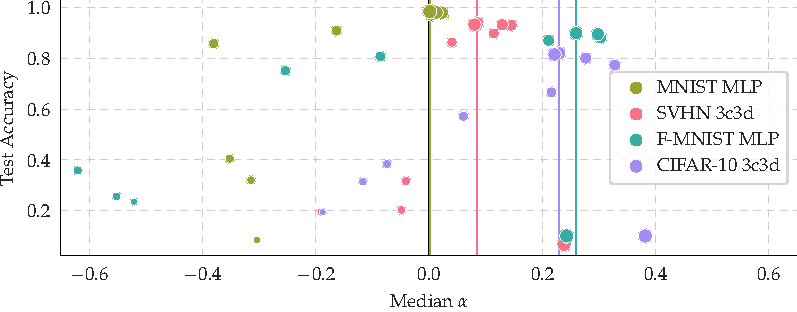
\includegraphics[width=\linewidth]{../repos/cockpit-paper/fig/07_learning_rate_selection/output/median_alpha_vs_performance_thesis-wide}
	\end{center}
  \vspace{-2ex}
	\caption{\textbf{Test accuracy as a function of standardized step size
      $\alpha$}. For four \deepobs problems (see \Cref{cockpit::app:benchmarks}), final
    test accuracy is shown versus the median $\alpha$-value over the entire
    training. Marker size indicates the magnitude of the raw learning rate,
    marker color identifies tasks (see legend). For each problem, the
    best-performing setting is highlighted by a vertical colored line.}
	\label{cockpit::fig:alpha_exp}
\end{figure*}

Across multiple optimization problems, we observe, perhaps surprisingly, that
the best runs and indeed all good runs have a median $\alpha>0$
(\Cref{cockpit::fig:alpha_exp}). This illustrates a fundamental difference between
stochastic optimization, as is typical for machine learning, and classic
deterministic optimization. Instead of locally stepping ``to the valley floor''
(optimal in the deterministic case), stochastic optimizers should
\emph{overshoot} the valley somewhat. This need to ``surf the walls'' has been
hypothesized before \citep[e.g.][]{wu2018understanding,xing2018walk} as a property of neural
network training. Frequently, learning rates are adapted during training, which
fits with our observation about positive $\alpha$-values: ``overshooting''
allows fast early progression towards areas of lower loss, but it does not yield
convergence in the end. Real-time visualizations of the training state, as
offered by \cockpit, can augment these fine-tuning processes.

\Cref{cockpit::fig:alpha_exp} also indicates a major challenge preventing simple
automated tuning solutions: the optimal $\alpha$-value is problem-dependent, and
simpler problems, such as a multi-layer perceptron (\mlp) on \mnist
\citep{lecun1998gradient}, behave much more similar to classic optimization problems.
Algorithmic research on small problems can thus produce misleading conclusions.
The figure also shows that the $\alpha$-gauge is not sufficient by itself:
extreme overshooting with a too-large learning rate leads to poor performance,
which however can be prevented by taking additional instruments into account.
This makes the case for the cockpit metaphor of increasing interpretability from
several instruments in conjunction. By combining the $\alpha$-instrument with
other gauges that capture the local geometry or network dynamics, the user can
better identify good choices of the learning rate and other hyperparameters.

%%% Local Variables:
%%% mode: latex
%%% TeX-master: "../thesis"
%%% End:
